\chapter{Cellbiologi}

Miljontals år av evolution har lett till att det idag finns en mängd olika sorters celler med sina egna inre strukturer. Det finns allt från bakteriers till synes oordnade inre till djur- och växtcellers högst strukturerade innanmäte. 

Cellerna måste både kunna hålla sig vid liv och reproducera sig för att deras gener ska leva vidare. Dessa uppgifter kan vidare delas upp i deluppgifter som tilldelas olika delar av cellens beståndsdelar. Om cellerna samverkar kan ett mer avancerat flercelligt liv upprätthållas. Då ställs större krav på ordning inom och mellan cellerna.

Resterande del av detta kapitel bygger huvudsakligen på information från boken \emph{The Cell} av G. M.  Cooper~\cite{Cooper_TheCell2000} om inget annat anges.


\section{Cytoplasman}
I studiet av levande organismer skiljer man på celler med sitt arvsanlag samlat i en cellkärna, eukaryoter, och de utan cellkärna, prokaryoter. Bakterier tillhör de sistnämnda medan svampar, växter och djur tillhör de förstnämnda. Cellen fyller dock många fler funktioner än att bara vara förvaringsplats för arvsmassan, och dessa egenskaper beror starkt på vilken miljö den anpassats till evolutionärt. De flesta celltyper har dock något slags skyddande hölje i form av cellvägg eller cellmembran och där innanför en vätska fylld med diverse filament, partiklar och en mängd olika organeller som var och en har sina specifika arbetsuppgifter. Denna blandning kallas med ett gemensamt namn för cytoplasman, illustrerat i \figref{fig:cell_struktur}

Organellerna varierar i storlek och koncentration och det finns allt från många mindre mitokondrier som ser till att maten vi förtär omvandlas till kroppens egna energikälla, ATP, till den stora strukturen av endoplasmatiska nätverket som bland annat syntetiserar proteiner. Förutom att bryta ner näringsämnen och från dem tillverka nya ämnen är en annan viktig process i cytoplasman transport, där en mängd olika organeller och strukturer inom cellen bidrar.


\begin{figure}\centering
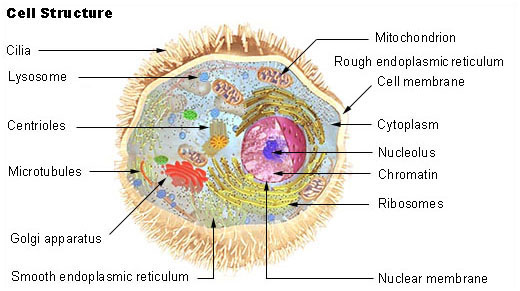
\includegraphics[width=0.7\textwidth]{bilder/Illu_cell_structure.jpg}
\caption{En eukaryot cells anatomi. Cytoplasman innehåller många olika organeller av varierande storlek. \footnotesize Bilden är allmän egendom\cite{wiki:illu_cell_structure} (en: public domain) och får därför reproduceras fritt.}
\label{fig:cell_struktur}
\end{figure}

%By OpenStax College [CC BY 3.0 (http://creativecommons.org/licenses/by/3.0)], via Wikimedia Commons

\subsection{Transport inom cellen}

Att partiklar, från små näringsämnen till stora proteiner, kan ta sig fram genom cytoplasman spelar onekligen en viktig roll för många funktioner i cellen. Om exempelvis näringen vi får från maten inte skulle nå cellernas energifabriker, mitokondrierna, tillräckligt snabbt eller komma fram i för liten skara skulle cellen med stor sannolikhet snabbt upphöra att fungera. Detta då många av cellens funktioner är starkt beroende av det ATP som mitokondrierna\footnotemark{} producerar.
\footnotetext{Även om en mindre mängd ATP kan produceras utan mitokondriernas hjälp. Dock bildas majoriteten av ATP:n just i mitokondrierna~\cite{Solunetti_ATP}.}

I celler definieras två typer av transport i cytoplasman: den aktiva och den passiva transporten. Under den aktiva transporten vandrar så kallade motorprotein längs med proteintrådar och för med sig det som ska transporteras. Under den passiva transporten tillåts ämnena diffundera fritt genom cytoplasman, vilket till skillnad från driften av motorproteinerna inte kräver energi. 
Vilket transportsystem som är dominerande beror på vilken celltyp som betraktas. I mer primitiva celltyper som bakterier och jästceller dominerar den passiva transporten medan det i celltyper som bildar stora, avancerade och sammanhängande organismer är vanligare med en dominant aktiv transport. Detta eftersom diffusion som transportprocess inte är tidseffektiv över stora avstånd.

Förutom aktinfilamenten som beskrivs i avsnittet nedan finns i cellen även lite tjockare proteintrådar kallade mikrotubuli. Dessa är inte symmetriska utan har en orientering där deras ena ände kallas ''$+$'' och den andra ''$-$''. Längs dessa proteintrådar kan motorprotein vandra samtidigt som de på sin ovansida fäster tag i något annat för att transportera detta längs med strängen. Det finns en typ av motorprotein som går från ''$+$'' till ''$-$'' och en annan typ som går åt motsatt håll. Dessa mikrotubuli sitter oftast ordnade i grupp med samma ände inåt. Detta möjliggör den aktiva transporten inom cellerna genom att rätt sorts motorprotein tillåts binda till det som behöver transporteras. 

%Förutom att transportera organeller och membranförslutna paket kan strukturen med dessa tjockare proteintrådar med rätt sorts motorproteiner även hålla vissa membranomslutna organeller på plats. Till exempel skulle Golgiapparaten, som är med och ser till att de syntiserade proteinerna i cellen hamnar på rätt plats, splittras upp i bitar och spridas runt i cellen om den inte hölls på plats mot cellens mitt av inåtvandrande motorproteiner. Även vid anafasen, som är en av faserna under celldelning där de duplicerade kromosomerna separeras så att de två sidorna av cellen får var sin kompletta uppsättning av dem, spelar mikrotubuli och motorproteiner en viktig roll.

Alla dessa proteintrådar skulle kunna påverka cytoplasmans genomtränglighet och i nuläget råder viss oenighet gällande hur cytoplasman egentligen ter sig för partiklar som rör sig genom den. Man har länge trott att cytoplasman upplevs olika beroende på partiklarnas storlek. Små partiklar upplever en kolloid vätskefas där de är väl blandade i cytoplasman medan större partiklar, på grund av sin storlek, ser cytoplasman som ett sammanhängande nätverk av interagerande komponenter. Det senare ger cytoplasman ett mer fast eller glasliknande tillstånd. Nya rön~\cite{Parry_etal2014} spekulerar dock i att dessa upplevda faser hos cytoplasman kan regleras och ändra karaktär.

Det finns även vissa teorier om att partikelrörelsen i celler skulle kunna påverkas av den sammanlagda effekten av motorproteinernas framryckningar. Även om dessa på liten skala ter sig väl riktade och ordnade kan den sammanlagda effekten av alla dessa transporter, tillsammans med turbulensen som bildas kring dem, resultera i en stokastisk kraft. På så sätt kan partikelns rörelsemönster påverkas stokastiskt av aktiv transport. 

Passiv transport i celler delas in i fyra processer: diffusion, underlättad diffusion, osmos och filtrering~\cite{Cram_Passivetransport}. Diffusion omfattar nettotransport av partiklar från områden av högre koncentration till områden med lägre koncentration. Underlättad diffusion sker för större partiklar, som av sig själva inte kan diffundera genom cellmembran. Transportproteiner i cellmembranet möjliggör dock denna transport som kan ske utan energitillförsel, det vill säga med koncentrationsgradienten. Diffusion av vatten genom membran anses vara en tillräckligt viktig process för att få ett eget namn, osmos. Filtrering sker för partiklar och vatten genom  porer i blodkärlsväggarna på grund av att trycket är högre i ådrorna än i omgivningen.


\subsection{Cellens olika faser}

Under odling av celler kommer kolonin genomgå tre distinkta faser~\cite{Heidcamp_Cellfas}. Initialt, under \emph{lag-fasen}, anpassar sig cellerna till omgivningen under vilket få nya celler produceras. Denna fas varar som mest någon dag och följs sedan av \emph{log-fasen} där celltillväxten sker exponentiellt. Denna fas pågår tills något näringsämne begränsar tillväxten. Om näringstillförseln är konstant avstannar tillväxten och cellantalet når en platå, \emph{stationärfas}. Denna fas kan även nås om utrymmet tillgängligt för kolonin är begränsat då tätt-packade celler inte delar sig. 
Om näring inte tillförs kommer istället cellantalet att minska och kolonin kommer in i \emph{dödsfasen}.

Utöver dessa faser kan vissa celltyper gå i dvala, en överlevnadsfas för tider då näringen är bristfällig eller klimatet ogynnsamt. Om man till exempel kyler ner jästceller kommer de att stänga ner icke-vitala processer för att dra ner på sin ämnesomsättning och därmed gå i dvala \cite{Postma_Dvala2009}. 


\section{Aktinfilament}

Aktinfilament, polymeriserat aktin även kallat F-aktin, skapas genom att fria aktinmonomerer, G-aktin, binds till varandra och bildar polymerer. Denna process kan ske spontant åt båda hållen i en aktinlösning och når då ett jämviktsläge. Utifrån en kort filamentbit kan alltså en längre kedja byggas upp, men på grund av att G-aktinet inte är helt symmetriskt utan har en orientering kommer tillväxten att ske snabbare i ena änden än den andra. Asymmetrin för de enskilda monomererna gör att hela filamentet i sig får en orientering vilket bland annat möjliggör dess användning som transportväg för motorproteiner. %Denna syntes av aktinfilament sker cirka 100 gånger snabbare inuti celler än utanför celler i laboratorium då cellen har hjälp av en mängd  katalyserande proteiner med både uppbyggande och nedbrytande egenskaper. Dessa proteiners aktivitet kan i sig regleras och fås att öka eller minska som respons på visst stimuli.

Varje G-aktin i filamenten sitter lite vridet i förhållande till sina grannar vilket leder till att filamenten får formen av en dubbelhelix med bredd på ca 7\,nm och upp till flera mikrometer långa. Dessa dubbelhelixar kan i sin tur kopplas samman av andra proteiner till mer avancerade 3-dimensionella strukturer.

Större delen av aktinfilamenten finns koncentrerade strax innanför cellmembranet. Där utgör de en del av cytoskelettet, ett nätverk som ger form och stadga till cellen samtidigt som det möjliggör viss transport. Detta nätverk har egenskaper liknande de som återfinns hos semisolida geler. Förutom att bilda 3-dimensionella nät kan aktinfilamenten även ordnas parallellt i mer tätpackade buntar. De tätast packade buntarna ger stöd åt utstickande strukturer från cellmembranet. De lite mer löst packade buntarna används tillsammans med motorprotein i strukturer som har förmågan att kontrahera, något som möjliggör sista steget i celldelningen där själva cellen delas i två. 

I denna rapport kommer aktinfilament även att betecknas som \emph{strängar}.
%Ett annat exempel är kroppens alla muskler som består av strukturer av aktintrådar och motorproteinet myosin.

%Som ett sista exempel kan nämnas att aktinfilament fyller en viktig funktion när cellen i sig förflyttar sig i sin omgivning. Cellen ändrar då form genom att skjuta fram ett utskott framför sig, fäster tag och drar sig fram en bit för att sedan upprepa processen.


\section{Jästceller}
%Datan som detta arbete bygger på kommer från observationer av partikelrörelse i jästceller, så här följer en kort introduktion till jäst. 

Jäst hör till riket svampar och utgörs av encelliga organismer~\cite{SGD_yeast}.
De finns på växter, i jorden men även på huden och i tarmkanalen hos varmblodiga djur. 
%Jästen kan där leva antingen i symbios med värddjuret eller som parasit och i värsta fall orsaka värddjuret skada. 
Att jäst är encelliga organismer möjliggör snabb reproduktion vilket gör dem smidiga att arbeta med i laboratorium. Dessutom uppvisar de större likhet med djurceller än de likväl encelliga bakterierna och ger därmed större möjlighet att dra paralleller till djurceller med försök på jästceller. 

\subsection{Jästcellers cytoplasma}
Att jästceller är svampar innebär att de därmed varken är djur, växter eller bakterier men delar vissa likheter med dessa tre celltyper. Med sitt arvsanlag samlat i en cellkärna~\cite{SGD_yeast}, precis som djur- och växtceller, skiljer sig jästceller från bakterier där arvsanlaget ligger blandat med resten av beståndsdelarna i cytoplasman.
De har även en vakuol och stabiliserande cellvägg som växtceller men saknar växtcellens kloroplaster och kan därmed inte utföra någon fotosyntes. Att jästcellen har en cellvägg innebär att den inte är lika beroende av ett stabiliserande proteinfilamentsnätverk och därmed endast har ett rudimentärt sådant~\cite{Midtveldt_etal2016}.

\subsection{Transport inom jästceller}
Djurcellernas komplicerade nät av proteintrådar, som möjliggör en aktiv transport inom cellen, finns inte hos jästceller~\cite{Midtveldt_etal2016} som istället får förlita sig på passiv transport, förutom vid celldelning. 
Med jästceller kan man därför undersöka om avvikelser från brownsk rörelse, som beskrivs i kommande kapitel, uppkommer även utan de stokastiska krafter med ursprung i det kollektiva bidraget från motorproteinerna.



\begin{comment}
%Om vi inte vill skriva en del om det som Daniels artikel kom fram till tror jag att det här avsnittet blir lite överflödigt.
\section{Det metabola tillståndets påverkan på partikelrörelse}
Tidigare studier~\cite{Gou_etal2014} på eukaryota celler har visat att
partiklars rörlighet i cytoplasman beror på hur aktiv cellen
är. Partikelrörligheten inuti, de i \cite{Gou_etal2014} undersökta, cellerna ökade exempelvis
trefaldigt om cellen drabbats av cancer jämfört med en normalt
fungerande cell. En cell som drabbats av cancer kommer att ha en förhöjd metabolism\cite{Gou_etal2014} för att öka på celldelningstakten, och kanske är det i samband med detta som även diffusionen i cytoplasman ökar. En möjlig förklaring till fenomenet utpekas i \cite{Gou_etal2014} vara icke-termiska fluktuationer orsakade av motorproteinernas sammanlagda aktivitet.

Studier~\cite{Parry_etal2014} på bakterier har samtidigt visat att
partiklarnas rörlighet minskade drastiskt om den metabola aktiviteten
minskade. Då bakterier saknar aktiv transport i sina celler försökte man här istället nå en förklaring där cytoplasman blir mer vätskelik ju högre aktiviteten är och börjar
likna ett mer elastiskt fast material då aktiviteten
minskar. Partikelstorleken tycks också vara en faktor för dess förmåga
att röra sig runt i cellen. I gränsen när partiklarna närmar sig
storleken av organellerna i cytoplasman blir förklaringen uppenbar;
partikeln kommer då på grund av sin storlek inte att kunna röra sig
runt i cellen som vid fri diffusion. 

Jästceller har förmågan att kunna gå i dvala, ett tillstånd där de
intracellulära aktiviteterna minskar. Då delar av den tillhandahållna
datan kommer från celler i dvala möjliggör detta undersökningar om
huruvida cytoplasmans beståndsdelars rörlighet i cellen även i detta arbete kan bekräftas bero på
cellens metabola tillstånd. 
\end{comment}

%Bara en liten kodsnutt som behövs när man kompilerar lokalt
%%% Local Variables: 
%%% mode: latex
%%% TeX-master: "00main.tex"
%%% End: 